% Notes:
% 
% The process of decomposing a two-way table (matrix) into two component
% matrices is called singular value decomposition (SVD), which is essentially the reverse process of
% matrix multiplication (from GGE
%
%
%
%
%

\documentclass[serif]{beamer}
% My beamer theme
\usetheme{Hannover}
\usecolortheme{crane}
\definecolor{gray10percent}{RGB}{229, 229, 229}
\definecolor{blockgray}{RGB}{198,188,169}

% My packages
\usepackage{amsmath}
\usepackage{graphicx}
\usepackage{rotating}
\usepackage{etoolbox}
\usepackage{xfrac} % for \sfrac{...}{...}
\usepackage{array} % for centered tabular

\usepackage{color}
\usepackage{listings}
\lstset
{
	language=C,
	captionpos=b,
	tabsize=3,
	keywordstyle=\color{blue},
	commentstyle=\color[rgb]{0.133,0.545,0.133},
	stringstyle=\color{red},
	breaklines=true,
	showstringspaces=false,
	basicstyle=\footnotesize,
	emph={label},
	keepspaces=true,
	emph={H,G,X,K,KPC},
    emphstyle={\bfseries}
}
\newcommand{\codepause}{\pause \vspace{-0.165in} } 
		
\newcommand\ConstrainedBox[3]{
  \makebox{\parbox[t][#1][c]{#2}{\centering#3}}}



% Decide if you want notes shown
\newtoggle{useNotes}
%\toggletrue{useNotes}
\togglefalse{useNotes}

\iftoggle{useNotes}
{
	\usepackage{pgfpages}
	\setbeameroption{show notes on second screen}
}


% Title Page definition
\title
{
	KPCA-Biplots
}
\subtitle{An implementation and further exploration}
\author
{
	Michael Semeniuk, Albert Steppi, and \linebreak
	Christopher Wolas
}
\date
{
	\begin{block}{}
	\begin{itemize}
		\item[~]
		{
			\underline{Mining Gene Expression Profiles: An Integrated} \linebreak
			\underline{Implementation of Kernel Principal Component} \linebreak
			\underline{Analysis and Singular Value Decomposition}
			\begin{itemize}
					\item[~]  Reverter et al,Genomics Proteomics Bioinformatics (2010)
			\end{itemize}
		}
	\end{itemize}	
	\end{block}
	
}

\begin{document}
	
	\section{Problem Domain}
	
	\begin{frame}
		\titlepage		
	\end{frame}

	\begin{frame}[t]
	\frametitle{Simplified Problem Domain Explanation}
		Understanding of our problem domain is as easy as... \linebreak
		\uncover<1-> {1, }
		\uncover<2-> {2, }
		\uncover<3>  {3}
		\begin{columns}[t]
		
			\column{2in}
			{
				\only<1>
				{
					\begin{block}
					{ 
						Analyze Microarray Expression Profiles Relationships
					}
					{
						Extract the highly \underline{non-linear} relationships
						between gene expression profiles and disease 
						classification using \textbf{modern machine learning} techniques.	
					}
					\end{block}
				}
				\only<2>
				{
					\begin{block}
						{ 
							Visualize These Relationships
						}
						{
							Use specialized graphs called \textbf{biplots}
							which plot \emph{both} the gene intensities and classifications on the same $R$-dimensional plane.
						}
					\end{block}
				}
				\only<3>
				{
					\begin{block}
					{
						Interepret relationships and focus on
						a specialized problem						
					}
					{
						\footnotesize 
						Find meaningful results such as:
						\begin{itemize}
							\item Gene Up/Down-\linebreak 
							Regulation in certain diseases
							\item Classifying novel Gene Profiles based on
							analyzed data
						\end{itemize}
						This \emph{can} lead to \underline{seperate} specialized
						research topics.
					}
					\end{block}
				}
			}
			\column{1in}
			{
				\only<1>
				{
					\begin{center}
						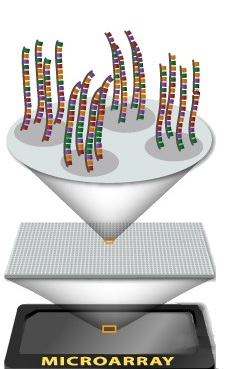
\includegraphics[width=1in]{images/microarray}	
					\end{center}
				}
				\only<2>
				{
					\vspace{0.5in}
					\textbf{IMAGE OF BIPLOT}
				}
				\only<3>
				{
					\vspace{-0.10in}
					\begin{center}
						
\includegraphics[width=1in]{images/meme_face}
					\end{center}
				}
			}
		\end{columns}
	\end{frame}
	
	\begin{frame}[t]
		\frametitle
		{
			``Microarray analysis? \linebreak
		}
		\framesubtitle
		{		
			\vspace{-0.2in}
			... Isn't that an ancient problem? \linebreak
			Why on earth would you do that...?!''
		
		}
		
		\begin{itemize}
			
			\item
			{
				\color<2-3>{gray10percent}
				{
					By using more sophisticated techniques (non-linear machine
					learning) we can extract \underline{higher fidelity results}
					on the same data which can lead to better insights.
				}
			}
			\item
			{
				\color<1,3>{gray10percent}
				{
					An \underline{approachable problem} that gives an
					introductory taste of bioinformatics for
					machine learning students unfamiliar with it.
				}
			}
			\item
			{
				\color<1-2>{gray10percent}
				{
					Problem in the realm of \underline{exploratory statistics}
					which help us understand the large and intricate data 
					we're working with.
				}
			}
		\end{itemize}
		
		
		\note
		{
			Dr. Hu made a comment on this being an old problem. Disspell
			any further implication that we're just doing a meaningless project
			that has no further value to be extracted from it.
		}
	\end{frame}
	
	\section{Algorithm}
	\subsection{Problem Specification}

	\begin{frame}
		\frametitle{KPCA-Biplot Algorithm}
		\framesubtitle{Problem Formulation}
		
		Start with a Gene Expression Profile matrix $\mathbf{X}$:

		% This is the crazy gene expression matrix with annotations
		\begin{equation}			
		\begin{matrix}
                            % Column anotation
		& & \mathbin
					{ 
						\color[rgb]{0.133,0.545,0.133}\text{Columns represent}
					} 
					& & \\
		& & \mathbin
					{
						\color[rgb]{0.133,0.545,0.133}\text{gene expression intensities}
					}
					& & \\
		& & \rotatebox[origin=c]{270}
			{
				$\begin{cases} 
				& \\ & \\ & \\ & \\ &  \\ & \\ &  \\  & \\ 
				\end{cases}$
			} 
		& & \\
		% Gene expression Matrix 'X'
		&\mathbf{X}=  
		&	\begin{bmatrix}
				x_{1,1} & x_{1,2} & x_{1,3} & \ldots  & x_{1,p} \\ 
				x_{2,1} & x_{2,2} & x_{2,3} & \ldots  & x_{2,p} \\ 
				x_{3,1} & x_{3,2} & x_{3,3} & \ldots  & x_{3,p} \\ 
				\vdots  & \vdots  & \vdots  & \ddots  &         \\ 
				x_{n,1} & x_{n,2} & x_{n,3} &         & x_{n,p} \\ 
			\end{bmatrix}
                            % Row Anotation
		&\left.
			\begin{matrix}
				\\ \\ \\ \\ \\  
			\end{matrix}
		 \right\}
        & \rotatebox[origin=c]{0}
        	 {
        	 	$\begin{matrix} 
                    \mathbin
                    {
                    	\color[rgb]{0.133,0.545,0.133}\text{Rows}
					  }\\
	          		  \mathbin
	          		  {
	          		  	\color[rgb]{0.133,0.545,0.133}\text{represent}
	          		  }\\
	          		  \mathbin
	          		  {
	          		  	\color[rgb]{0.133,0.545,0.133}\text{labeled}
	          		  } \\ 
	          		  \mathbin
	          		  {
	          		  	\color[rgb]{0.133,0.545,0.133}\text{samples}
	          		  } \\ 
          		  \end{matrix}$
      		  } \\

		\end{matrix}
		\end{equation}
		
	\end{frame}
	
	\begin{frame}
		\frametitle{}
			\begin{block}{Terminology Notes:}
			\begin{itemize}
				\item 
				{
					\color<2,3>{blockgray}
					{
						Gene expression intensities are measurements
						of the activity of each gene.\newline
					}
				}
				\item 
				{
					\color<1>{blockgray}
					{
						They can tell us:
					}
					
					% WOW, this is super wordy. I want to say this more succinctly.
					% Explain what a condition could be: Abnormality, Disease, Syndrome, identifiable trait(?)
					\begin{enumerate}
						\item
						{
							\color<1,3>{blockgray}
							{
								Upregulation or downregulation of genes
								depending if certain condition is expressed.
							}
						}
						\item
						{				
							\color<1,2>{blockgray}
							{
								Collectively, they can form gene expression
								profiles which can identify an indivdual 
								with a condition.
						    }
						}
					\end{enumerate}
				}
			\end{itemize}
				
				
			\end{block}
			
	\end{frame}
	
	\subsection{Preprocessing}
	
	\begin{frame}[fragile,t]
		\frametitle{KPCA-Biplot Algorithm}
		\framesubtitle{Preprocessing}
		Next, perform preprocessing. \newline

		\begin{lstlisting}[mathescape]
		for(i $\ldots$ N)
		{
		    // Where $\mathbin{ \color[rgb]{0.133,0.545,0.133} T_{i}}$(...) is some preprocessing function
		    // which transforms a vector into a new one.	
		    $\mathbf{X}=T_{i}(\mathbf{X})$
		}
		\end{lstlisting}	
		
		\note
		{

		}
	\end{frame}

	\begin{frame}
		\begin{block}{Notes:}
			
			Several established techniques are as follows:
			
			\begin{enumerate}
				\item
				{
					\color<2->{blockgray}
					{
						Normalization (e.g. $\log$ transformation)
					}
				}
				\item
				{	
					\color<1,3->{blockgray}
					{					
						Gene Centering (subtract $\mu$
						intensity of gene from each gene)
					}
				}
				\item
				{
					\color<1-2,4->{blockgray}
					{
						Gene Scaling (by standard deviation)
					}
				}
				\item
				{
					\color<1-3,5>{blockgray}
					{
						Filters
					}
					\begin{enumerate}
						\item
						{
							\color<1-3,5>{blockgray}
							{
								Simple threshold filters
							}
						}
						\item 
						{
							\color<1-3,5>{blockgray}
							{
								Interquartile Range filters
							}
						}
						\item
						{
							\color<1-3,5>{blockgray}
							{
								ANOVA fitlers
							}
						}
					\end{enumerate}
				}
				\item 
				{
					\color<1-4>{blockgray}
					{
						Sample Removal
					}
					\begin{enumerate}
						\item
						{
							\color<1-4>{blockgray}
							{
								Errorneous samples
							}
						}
						\item
						{
							\color<1-4>{blockgray}
							{
								Incomplete samples
							}
						}
						\item
						{
							\color<1-4>{blockgray}
							{
								Sample of a classification with not enough samples
							}
						}
					\end{enumerate}
				}
			\end{enumerate}
		\end{block}
		
	\end{frame}

	\subsection{SVD}

	\begin{frame}[fragile,t]
		\frametitle{KPCA-Biplot Algorithm}
		\framesubtitle{Singular Value Decomposition \textbf{(SVD)}}
		Now perform singular value decomposition. \newline
		
		
		\begin{lstlisting}[mathescape, language=C]
		// Decompose matrix X into 3 parts using SVD:
		// U = Unitary matrix
		\end{lstlisting}
		\codepause
		\begin{lstlisting}[mathescape, language=C]
		// D = rectangular diagonal matrix (with
		//       positive real numbers)
		\end{lstlisting}
		\codepause 
		\begin{lstlisting}[mathescape, language=C]
		// $\mathbin{ \color[rgb]{0.133,0.545,0.133} V^{T}}$ = conjugate transpose of V (a unitary matrix)
		\end{lstlisting}
		\codepause
		\begin{lstlisting}[mathescape, language=C]
		$ U D V^{T} =$ X
		\end{lstlisting}
		\codepause
		\begin{lstlisting}[mathescape, language=C]
		
		// Get the expression in terms of G and H:
		GH$^{T}$ = $U D^{\alpha} D^{(1 - \alpha)} V^{T}$ = $U D V^{T}$ = X 
		\end{lstlisting}
		\codepause
		\begin{lstlisting}[mathescape, language=C]
		
		// Decompos. of Rows Effects (Microarray Samples):
		G = $U \times D^{\alpha}$ 	
		\end{lstlisting}
		\codepause
		\begin{lstlisting}[mathescape, language=C]
		
		// Decompos. of Column Effects (Gene Expressions):
		H$^{T}$ = $V^{T} \times D^{(1-\alpha)}$	
		\end{lstlisting}
	\end{frame}

	\begin{frame}
		\begin{block}{TODO SVD:}
			\begin{itemize}
				\item  Explain SVD (high level with perhaps some math and handwaving)
				\item  visualization of SVD (in terms of affine transforms)
				\item  I like http://nimbledais.com/?p=57
			\end{itemize}
		\end{block}
		\begin{center}
			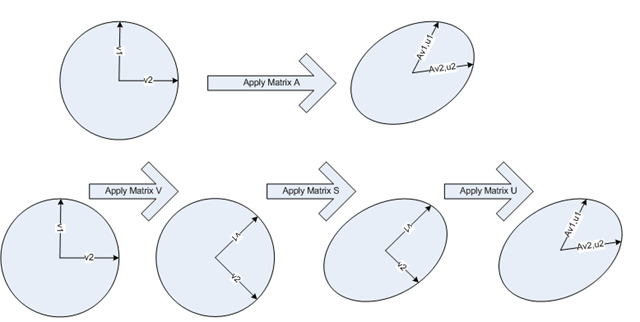
\includegraphics[width=2in]{images/svd_intuitive}	
		\end{center}
		
	\end{frame}
	
	\begin{frame}
		\begin{block}{TODO $\alpha$:}
			Explain $\alpha$ and its purpose
		\end{block}
	\end{frame}
	
	\subsection{Kernel Matrix}
	
	\begin{frame}[t, fragile]
		\frametitle{KPCA-Biplot Algorithm}
		\framesubtitle{Finding the Kernel Matrix}
		
		Compute the Kernel Matrix.
		
		\begin{lstlisting}[mathescape, language=C]
		
		// Use the radial basis kernel which takes the form:
		//  $\mathbin{ \color[rgb]{0.133,0.545,0.133} K(x,y) = exp(-\frac{{ \left\| x-y \right\|  }^{ 2 }}{2\sigma^{2}})}$
		// 
		// 
		//
		//
		//
		//
		\end{lstlisting}
		% Let's be clever and make an image comment lol
		\vspace{-1.10in}
		\begin{center}
		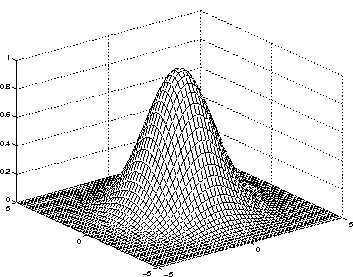
\includegraphics[width=1.0in]{images/rbf_kernel}	
		\end{center}
		\vspace{-0.07in}
		\codepause
		\begin{lstlisting}[mathescape, language=C]
		// We will be computing the kernel matrix using our
		// radial basis kernel for H (the gene expressions)
		K = Find_Kernel_Matrix(kernel_function=$K_{\text{radial basis}}(x,y)$,
		                       dataset=H,
		                       $\sigma$ = To be determined )
		
		\end{lstlisting}

	\end{frame}
	
	\begin{frame}
		\begin{block}{Notes on Kernel:}
			% Quoting paper
			\begin{itemize}
			\item
			{
			\color<2-4>{blockgray}
			{
				Kernel function choice is critical since the kernel
				uses it as a similarity metric.
			}
				\begin{itemize}
					\item
					{
						\color<1,3-4>{blockgray}
						{
							Two natural candidates were considered:
						}
							\begin{enumerate}
							
								\item
								{ 
									\color<1,3-4>{blockgray}{Polynomial Kernel}
								}
								\item
								{ 
									\color<1,3-4>{blockgray}{Radial Basis Kernel}
								}
							\end{enumerate}
						
					}
					\item
					{
						\color<1-2,4>{blockgray}
						{
							\textbf{Radial Basis Kernel} was found 
							to do \underline{better} and is used.
						}
					}
				\end{itemize}
			}
			\item
			{
				\color<1-3>{blockgray}
				{
					Kernel tuning parameters are also \underline{critical} 
					(e.g. $\sigma$ value). This will be further 
					explored \emph{later}.
				}
			}
			\end{itemize}
		\end{block}
	\end{frame}
	
	\subsection{KPCA}
	
	\begin{frame}[t, fragile]
		\frametitle{KPCA-Biplot Algorithm}
		\framesubtitle{Kernel Principal Component Analysis \textbf{(KPCA)}}
		
		Perform Kernel Principal Component Analysis.
		
	\begin{lstlisting}[mathescape, language=C]
		// Extract the nonlinear features of gene expression 
		// matrix H by computing the first 2 principal 
		// components using the Kernel Matrix
		KPC$_{H}$ = Do_KPCA(num_of_principal_components = 2,
		               kernel_matrix = K)
	\end{lstlisting}

	\end{frame}

	\begin{frame}
		\begin{block}{KPCA TODO:}
			\begin{itemize}
			\item  Some explanation of PCA (intuitive but mathematical, perhaps)
			\item  Extension from PCA to KPCA
			\item  Explanation of why \emph{2} Kernel Principal Components (visualizable graphical output)	
			\end{itemize}
		\end{block}
	\end{frame}

	\subsection{Projection}
	
	\begin{frame}[t, fragile]
		\frametitle{KPCA-Biplot Algorithm}
		\framesubtitle{Subspace Projection}
		
		\begin{lstlisting}[mathescape, language=C]
		// Compute a second Kernel Matrix for both the Gene
		...
		\end{lstlisting}
		\codepause
		\begin{lstlisting}[mathescape, language=C]
		
		// Project the microarrays G onto the subspace
		G$_{Projection}$ = K$^{T} \times $ KPC$_{ H }$
		\end{lstlisting}		
	\end{frame}
	
	\begin{frame}
		\begin{block}{Subspace Projection TODO:}
			\begin{itemize}
				\item  Write how it works
			\end{itemize}
		\end{block}
	\end{frame}
	
	\subsection{Biplot}

	\begin{frame}[t, fragile]
		\frametitle{KPCA-Biplot Algorithm}
		\framesubtitle{Plotting the Biplot}
		
		\begin{lstlisting}[mathescape, language=C]
		
		// Classification of each microarray sample row
		File$_{Classification}$ = Read_Classifications(...)
		\end{lstlisting}
		\codepause
		\begin{lstlisting}[mathescape, language=C]
		
		// Metadata about each gene column
		File$_{Genes}$= Read_Gene_Metadata(...)
		\end{lstlisting}
		\codepause
		\begin{lstlisting}[mathescape, language=C]
		
		// Plot your biplot with the collected data
		GE_Biplot(gene_expressions = G$_{Proj}$,
		          gene_metadata = File$_{Genes}$=,
		          microarray_samples = H,
		          microarray_classification = File$_{Classification}$)
		\end{lstlisting}
		\begin{lstlisting}[mathescape, language=C]
		>>
		>>
		>>
		>> 
		>>
		>>
		\end{lstlisting}
		% Let's be clever and make an image comment lol
		\vspace{-1.17in}
		\begin{center}
		\raggedright \hspace{0.2in}
		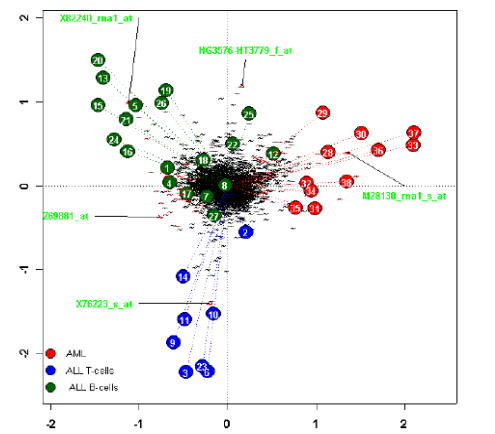
\includegraphics[width=1.0in]{images/biplot_output}	
		\end{center}
		\codepause
		
		
	\end{frame}
	
	\section{Datasets}
	\begin{frame}[t]
		\frametitle{Datasets}

		\begin{block}{\vspace{-0.5in}	}		
			In our research we've used {\bf 4} freely available datasets with labeled samples.
		\end{block}

		% http://icos.cs.nott.ac.uk/datasets/microarray.html
		% http://www.inf.ed.ac.uk/teaching/courses/dme/html/datasets0405.html
		
		\only<1>
		{
		\begin{enumerate}
	 		\setcounter{enumi}{0}
			\item {\bf COLON dataset}: 
				\begin{itemize}
					\item  $ Labels: \left \{ \textsc{ Tumor}, \textsc{ No Tumor}  \right \}$
					\item 2,000 gene expression levels
					\item  62 samples
					\begin{itemize}
						\item[$\rightarrow$] How many tumor
						\item[$\rightarrow$] How many not tumor
					\end{itemize}
					\item  \textsc{Preprocessing:}
					\begin{itemize}
						\item[$\rightarrow$] Item 1
						\item[$\rightarrow$] Item 2
						\item[$\rightarrow$] Item 3
					\end{itemize}
				\end{itemize}
		\end{enumerate}
		}
		\only<2>
		{
		\begin{enumerate}
	 		\setcounter{enumi}{1}
			\item {\bf LYMPHOMA dataset}: 
				\begin{itemize}
					\item  $ Labels: 
						\left \{ \textsc{DLBCL}\footnote{Diffuse large B-cell lymphoma},
							 \textsc{FL}\footnote{Follicular lymphoma}  \right \}$
					\item 6,817 gene expression levels
					\item 77 samples
					\begin{itemize}
						\item[$\rightarrow$] \textsc{DLBCL} Samples: 58
						\item[$\rightarrow$] \textsc{FL} Samples: 19
					\end{itemize}
					\item  \textsc{Preprocessing:}
					\begin{itemize}
						\item[$\rightarrow$]  Rescaling (multiply each sample by $\sfrac{1}{slope}$ of
						a linear least squares fit of the sample vs. the first sample "reference")
						\item[$\rightarrow$]  Minimum Thresholding at 20 (minimize noise effects)
						\item[$\rightarrow$]  Maximum Thresholding at 1600 (reduce florescence saturation)
						\item[$\rightarrow$]  Variation Filter (exclude genes with less than 3-fold variation and less than 100 units of standard deviation)
					\end{itemize}
				\end{itemize}
		\end{enumerate}
		}
		\only<3>
		{
		\begin{enumerate}
			\setcounter{enumi}{2}
			\item {\bf PROSTATE dataset}:
				\begin{itemize}
					\item  $ Labels: \left \{ \text{Tumor}, \text{No Tumor}  \right \}$
					\item 2,135 gene expression levels
					\item  77 samples
					\begin{itemize}
						\item[$\rightarrow$]  \textsc{Tumor} Samples: 52
						\item[$\rightarrow$]  \textsc{No Tumor} Samples: 50
					\end{itemize}					
					\item  \textsc{Preprocessing:}
					\begin{itemize}
						\item[$\rightarrow$]  Scaling (median of the mean difference of all genes)
						\item[$\rightarrow$]  Minimum Thresholding at 10
						\item[$\rightarrow$]  Maximum Thresholding at 1600
					\end{itemize}
				\end{itemize}
		\end{enumerate}
		}
		\only<4>
		{
		\begin{enumerate}
			\setcounter{enumi}{3}
			% http://www.biolab.si/supp/bi-cancer/projections/info/leukemia.htm
			\item {\bf Leukemia dataset}:
					\begin{itemize}
					\item  $ Labels: 	\left
						 \{ \text{ALL}\footnote{Acute lymphoblastic leukemia},
						 \text{AML}\footnote{Acute myeloid leukemia}
								 \right \}$
					\item 5,147 gene expression levels
					\item 72 samples
					\begin{itemize}
						\item[$\rightarrow$] \textsc{ALL} Samples: 47
						\item[$\rightarrow$] \textsc{AML} Samples: 25
					\end{itemize}
					\item  \textsc{Preprocessing:}
					\begin{itemize}
						\item[$\rightarrow$] Item 1
						\item[$\rightarrow$] Item 2
						\item[$\rightarrow$] Item 3
					\end{itemize}
				\end{itemize}
		\end{enumerate}		
		}
	\end{frame}

	\subsection{Tuning}
	\begin{frame}
		\begin{center}
			\huge
			``Wait a minute, what about the unsolved parameters?"
		\end{center}
	\end{frame}
	
	\begin{frame}
		\begin{block}{Optimization Parameters:}
			\begin{itemize}
				\item  $\alpha$ - ...
				\item  $\sigma$ - ...
			\end{itemize}
		\end{block}	
	\end{frame}
	
		
		\newcommand{\alphabiplot}[2]
		{
			\begin{center}
				\includegraphics[width=2.50in, height=2.50in]{images/alpha_graphs/#1}
				\linebreak
				{\huge $\alpha = #2$}
			\end{center}
		}
	
		% Save some monotony
		\newcommand{\sidealphabiplot}[2]
		{
			\begin{center}
				\includegraphics[width=0.75in, height=0.75in]{images/alpha_graphs/#1}
				\linebreak
				$\alpha = #2$
			\end{center}
		}
		\newcommand{\sidealphaspacer}
		{
			\begin{center}
				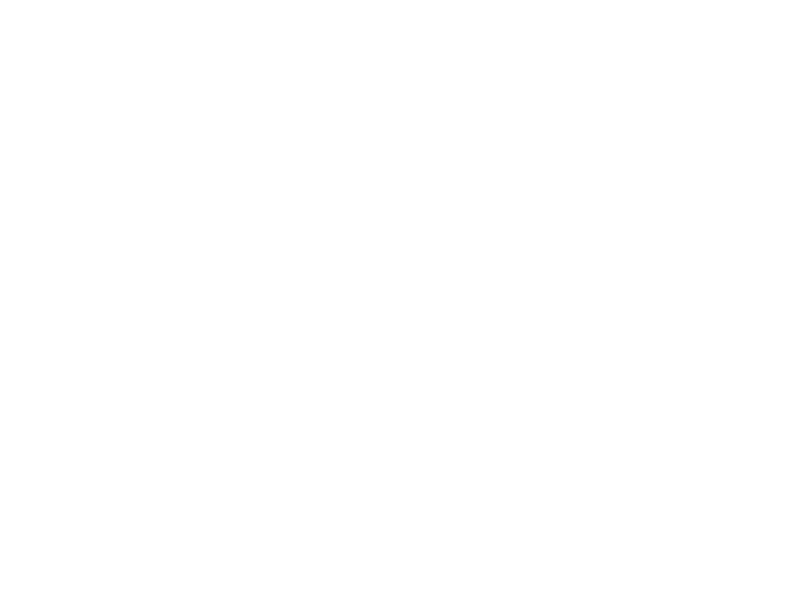
\includegraphics[width=0.75in, height=0.75in]{images/alpha_graphs/spacer}
				\newline
			\end{center}
		}
		\newcommand{\sidealphaboldbiplot}[2]
		{
			\begin{center}
				\includegraphics[width=0.75in, height=0.75in]{images/alpha_graphs/#1}
				\linebreak
				$\alpha = \textbf{#2}$
			\end{center}
		}

	
	\begin{frame}
	
	
		
	
		\begin{columns}
			\begin{column}{1in}
				% alpha = 0.00
				\only<1>
				{
					\sidealphaspacer
					\sidealphaboldbiplot{0_00}{0.00}
					\sidealphabiplot{0_10}{0.10}
				}
				% alpha = 0.10
				\only<2>
				{
					\sidealphabiplot{0_00}{0.00}
					\sidealphaboldbiplot{0_10}{0.10}
					\sidealphabiplot{0_20}{0.20}
				}
				% alpha = 0.20
				\only<3>
				{
					\sidealphabiplot{0_10}{0.10}
					\sidealphaboldbiplot{0_20}{0.20}
					\sidealphabiplot{0_30}{0.30}
				}
				% alpha = 0.30
				\only<4>
				{
					\sidealphabiplot{0_20}{0.20}
					\sidealphaboldbiplot{0_30}{0.30}
					\sidealphabiplot{0_40}{0.40}
				}
				% alpha = 0.40
				\only<5>
				{
					\sidealphabiplot{0_30}{0.30}
					\sidealphaboldbiplot{0_40}{0.40}
					\sidealphabiplot{0_50}{0.50}
				}
				% alpha = 0.50
				\only<6>
				{
					\sidealphabiplot{0_40}{0.40}
					\sidealphaboldbiplot{0_50}{0.50}
					\sidealphabiplot{0_60}{0.60}
				}
				% alpha = 0.60
				\only<7>
				{
					\sidealphabiplot{0_50}{0.50}
					\sidealphaboldbiplot{0_60}{0.60}
					\sidealphabiplot{0_70}{0.70}
				}
				% alpha = 0.70
				\only<8>
				{
					\sidealphabiplot{0_60}{0.60}
					\sidealphaboldbiplot{0_70}{0.70}
					\sidealphabiplot{0_80}{0.80}
				}
				% alpha = 0.80
				\only<9>
				{
					\sidealphabiplot{0_70}{0.70}
					\sidealphaboldbiplot{0_80}{0.80}
					\sidealphabiplot{0_90}{0.90}
				}
				% alpha 0.90
				\only<10>
				{
					\sidealphabiplot{0_80}{0.80}
					\sidealphaboldbiplot{0_90}{0.90}
					\sidealphabiplot{1_00}{1.00}
					
				}
				% alpha 1.00
				\only<11>
				{
					\sidealphabiplot{0_90}{0.90}
					\sidealphaboldbiplot{1_00}{1.00}
					\sidealphaspacer
				}
			\end{column}
			\begin{column}{3in}
				
				\only<1>{ \alphabiplot{0_00}{0.00} }
				\only<2>{ \alphabiplot{0_10}{0.10} }
				\only<3>{ \alphabiplot{0_20}{0.20} }
				\only<4>{ \alphabiplot{0_30}{0.30} }
				\only<5>{ \alphabiplot{0_40}{0.40} }
				\only<6>{ \alphabiplot{0_50}{0.50} }
				\only<7>{ \alphabiplot{0_60}{0.60} }
				\only<8>{ \alphabiplot{0_70}{0.70} }
				\only<9>{ \alphabiplot{0_80}{0.80} }
				\only<10>{ \alphabiplot{0_90}{0.90} }
				\only<11>{ \alphabiplot{1_00}{1.00} }
				
			\end{column}


		\end{columns}
	
	\end{frame}

	\begin{frame}
		
		\begin{table}
		\begin{tabular}
		{
			|>{\centering\arraybackslash}m{1.50in}
			|>{\centering\arraybackslash}m{1.00in}
			|>{\centering\arraybackslash}m{1.00in}|
		}
			\hline
				~ &
				\textbf{Reverter et Al.} &
				\textbf{Wolas et Al.} \newline (Us)
				
			\\
			\hline
				\textbf{COLON} &
				0.50 &
				0.50
			\\
			\hline
				\textbf{LYMPHOMA} &
				0.50 &
				0.50
			\\
			\hline
				\textbf{PROSTATE} &
				- &
				0.50
			\\
			\hline
				\textbf{LEUKEMIA} &
				0.50 &
				0.50  
			\\
			\hline
		\end{tabular}
		\caption{ $\alpha$ values for biplot}
	\end{table}
		
	\end{frame}

	\subsection{Validation}
	\begin{frame}
		Discussion of kernel tuning and cross validation 
	\end{frame}
	
	\begin{frame}
		Insert pseudocode for cross validation algorithm
	\end{frame}
	
	\begin{frame}
		
		\begin{table}
		\begin{tabular}
		{
			|>{\centering\arraybackslash}m{1.50in}
			|>{\centering\arraybackslash}m{1.00in}
			|>{\centering\arraybackslash}m{1.00in}|
		}
			\hline
				~ &
				\textbf{Reverter et Al.} &
				\textbf{Wolas et Al.} \newline (Us)
				
			\\
			\hline
				\textbf{COLON} &
				0.10 &
				- 
			\\
			\hline
				\textbf{LYMPHOMA} &
				0.01 &
				-
			\\
			\hline
				\textbf{PROSTATE} &
				- &
				- 
			\\
			\hline
				\textbf{LEUKEMIA} &
				0.001 &
				- 
			\\
			\hline
		\end{tabular}
		\caption{Optimized $\sigma$ for kernel}
	\end{table}
		
	\end{frame}
	
	
	\section{Results}
	
	\begin{frame}[t]

		\begin{block}
		{
			\only<1-2>
			{
				TUMOR Dataset
			}
			\only<3-4>
			{
				LEUKEMIA Datasets
			}
			\only<5>
			{
				PROSTATE Datasts
			}
			\only<6>
			{
				LYMPHOMA Dataset
			}
		}
		{
			TODO:Compare two graphs
		}	
		\end{block}

		\begin{columns}
			\begin{column}{1.75in}
				\vspace{-1.00in}
				
				\only<1-2>
				{
					\begin{center}
						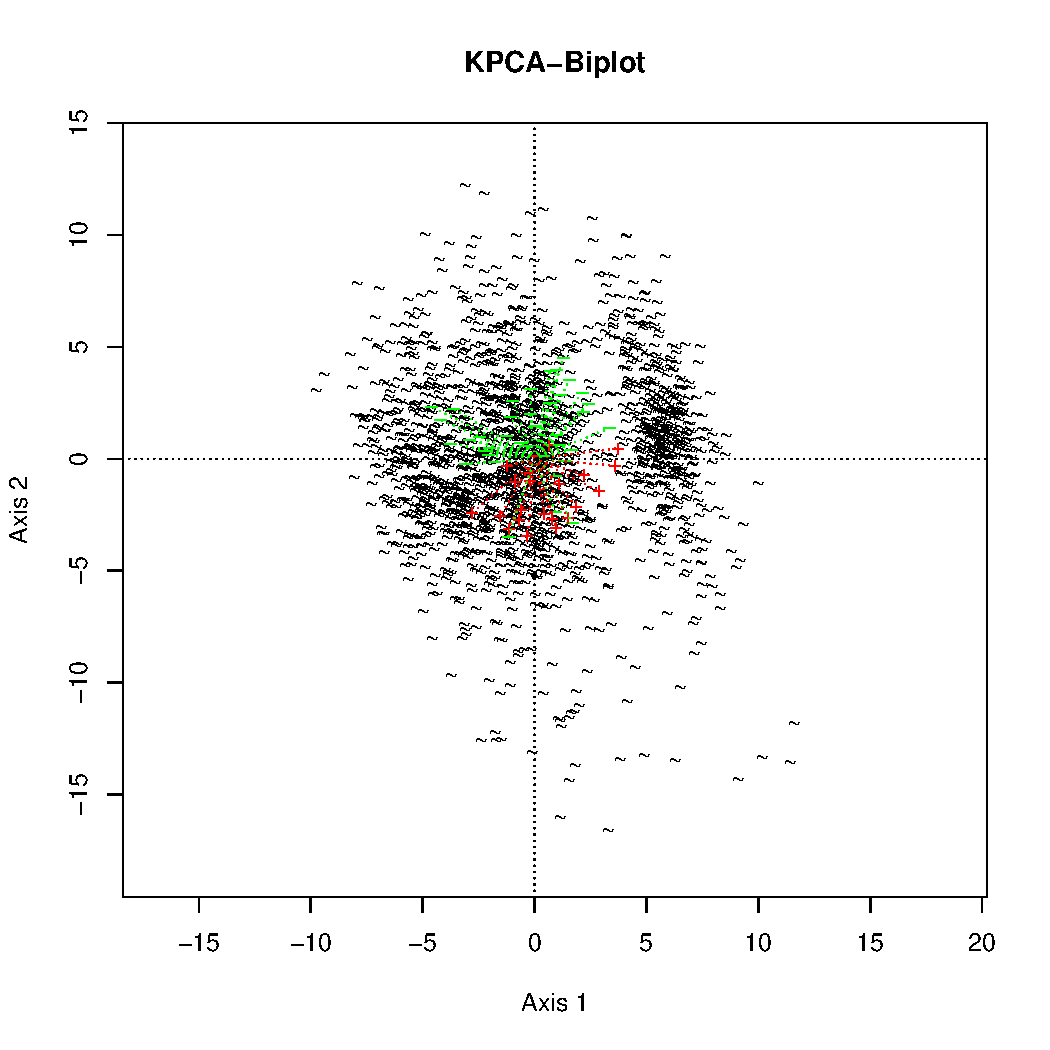
\includegraphics[width=1.5in, height=1.5in]{images/final_graphs/COLON_OUR_KPCA_BIPLOT}\newline
						\ConstrainedBox{0.25in}{1.75in}
						{
							Our KPCA-Biplot
						}
					\end{center}
				}
				\only<3-4>
				{
					\begin{center}
						
\includegraphics[width=1.5in, height=1.5in]{images/final_graphs/LEUKEMIA_OUR_KPCA_BIPLOT}\newline
						\ConstrainedBox{0.25in}{1.75in}
						{
							Our KPCA-Biplot
						}
					\end{center}
				}
				\only<5>
				{
					\begin{center}
						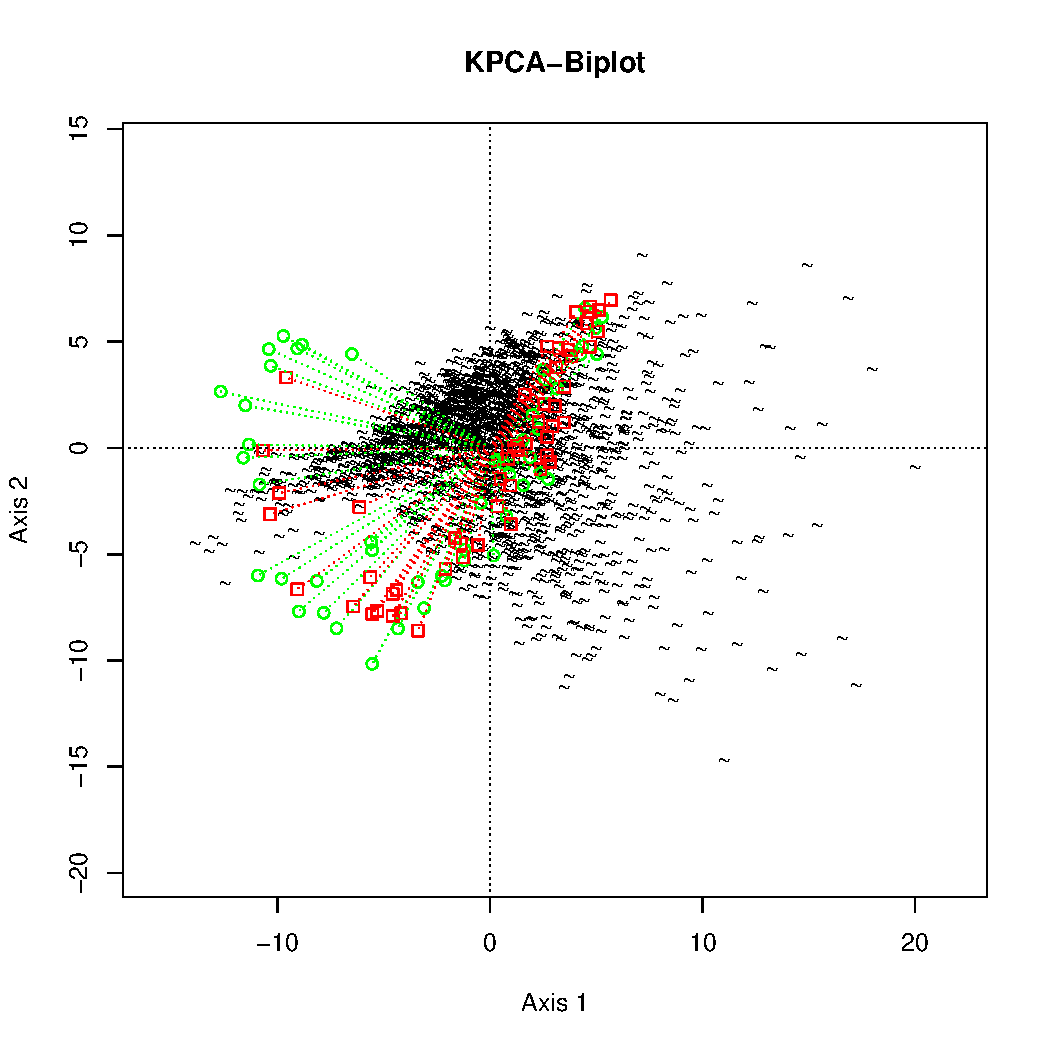
\includegraphics[width=1.5in, height=1.5in]{images/final_graphs/PROSTATE_OUR_KPCA_BIPLOT}\newline
						\ConstrainedBox{0.25in}{1.75in}
						{
							Our KPCA-Biplot
						}
					\end{center}
				}
				\only<6>
				{
					\begin{center}
						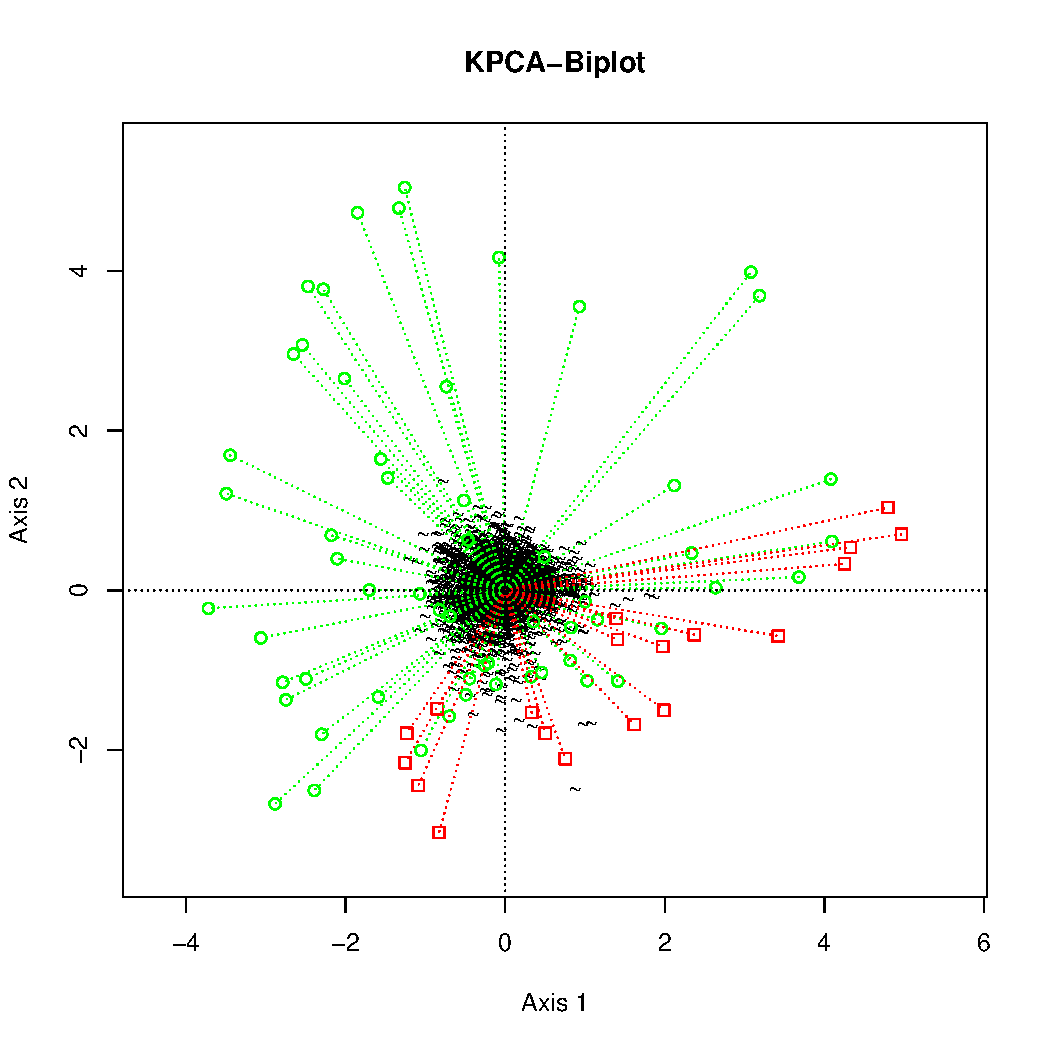
\includegraphics[width=1.5in, height=1.5in]{images/final_graphs/LYMPHOMA_OUR_KPCA_BIPLOT}\newline
						\ConstrainedBox{0.25in}{1.75in}
						{
							Our KPCA-Biplot
						}
					\end{center}
				}
				
				
			\end{column}
			\begin{column}{0.5in}
				\begin{center}
					\vspace{-0.50in}
					\ConstrainedBox{0.50in}{0.50in}
					{
						\huge \textbf{VS.}
					}
					
				\end{center}
			\end{column}
			\begin{column}{1.75in}
				\vspace{0.75in}
				%
				% COLON
				%
				\only<1>
				{
					\begin{center}
						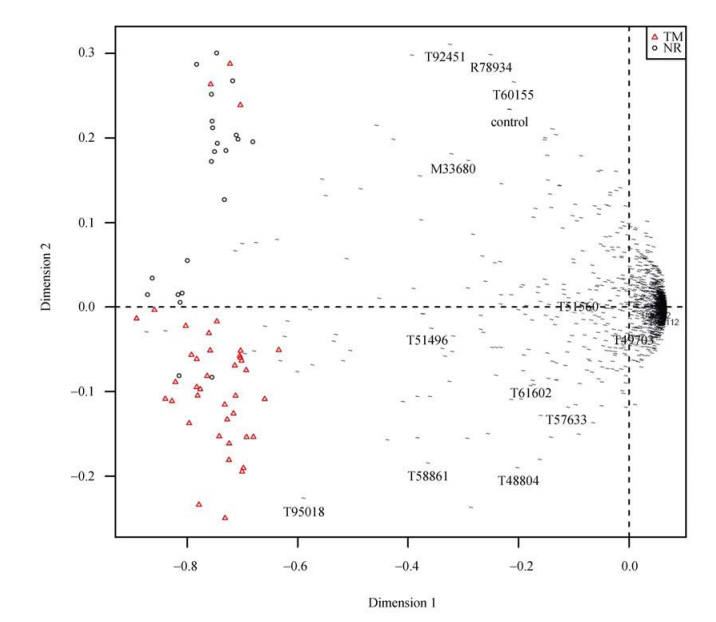
\includegraphics[width=1.5in, height=1.5in]{images/final_graphs/COLON_REVERTER_KPCA_BIPLOT}\newline
						\ConstrainedBox{0.25in}{1.75in}
						{
							Reverter et Al.
							KPCA-Biplot
						}
					\end{center}
				}
				\only<2>
				{
					\begin{center}
						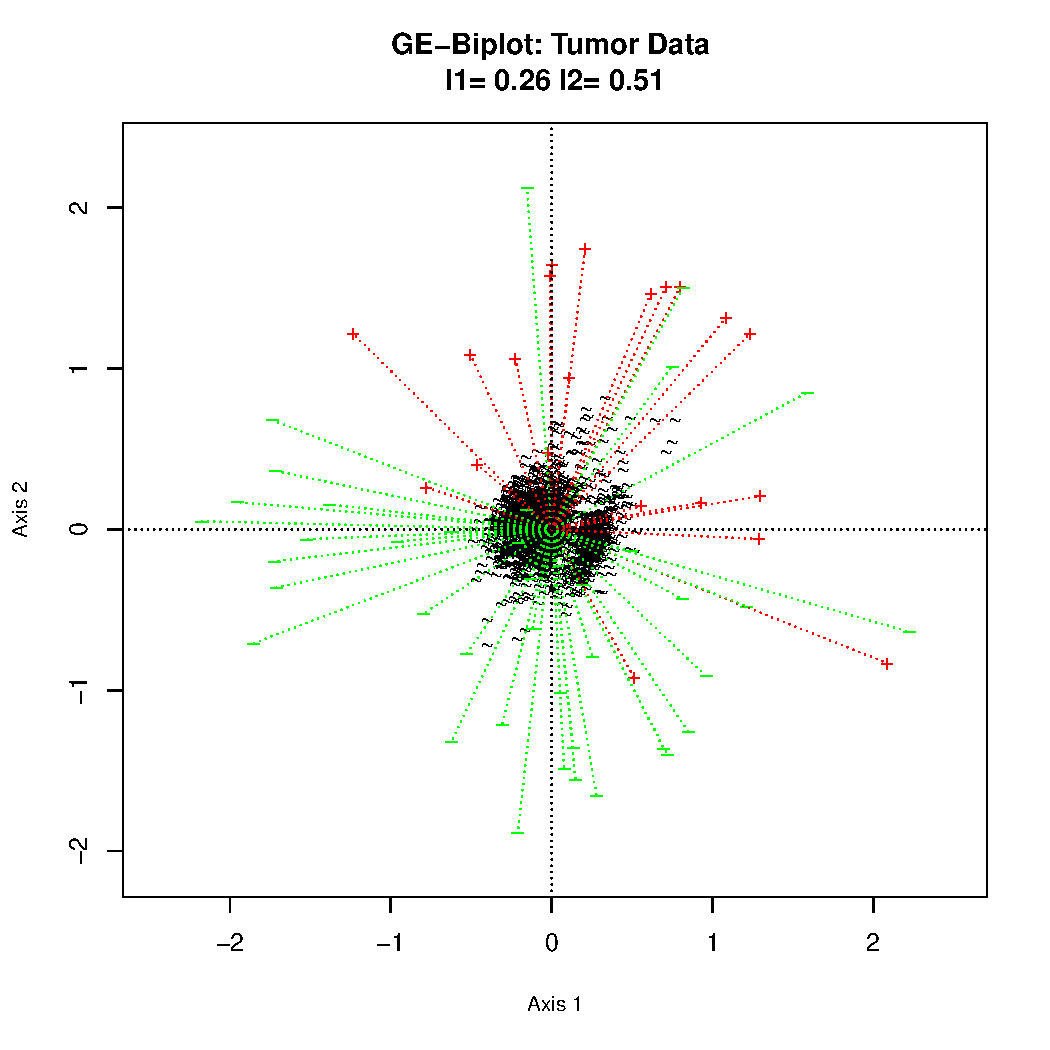
\includegraphics[width=1.5in, height=1.5in]{images/final_graphs/COLON_BIPLOT}\newline
						\ConstrainedBox{0.25in}{1.75in}
						{
							Standard Biplot
						}
					\end{center}
				}
				%
				% LYMPHOMA
				%
				\only<3>
				{
					\begin{center}
						
\includegraphics[width=1.5in, height=1.5in]{images/final_graphs/LEUKEMIA_REVERTER_KPCA_BIPLOT}\newline
						\ConstrainedBox{0.25in}{1.75in}
						{
							Reverter et Al.
							KPCA-Biplot
						}
						
					\end{center}
				}
				\only<4>
				{
					\begin{center}
						
\includegraphics[width=1.5in, height=1.5in]{images/final_graphs/LEUKEMIA_BIPLOT}\newline
						\ConstrainedBox{0.25in}{1.75in}
						{
							Standard Biplot
						}
						
					\end{center}
				}
				\only<5>
				{
					\begin{center}
						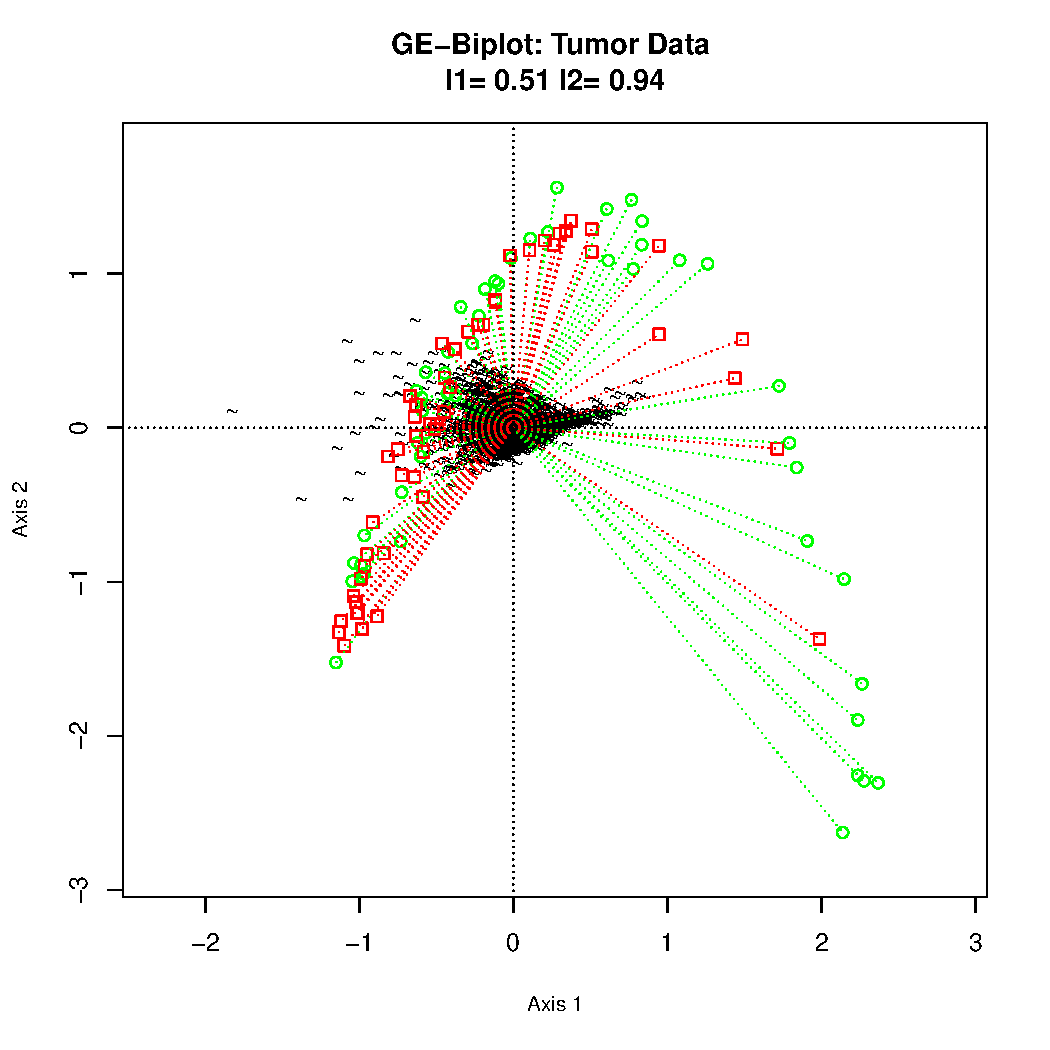
\includegraphics[width=1.5in, height=1.5in]{images/final_graphs/PROSTATE_BIPLOT}\newline
						\ConstrainedBox{0.25in}{1.75in}
						{
							Standard Biplot
						}
					\end{center}
				}
				\only<6>
				{
					\begin{center}
						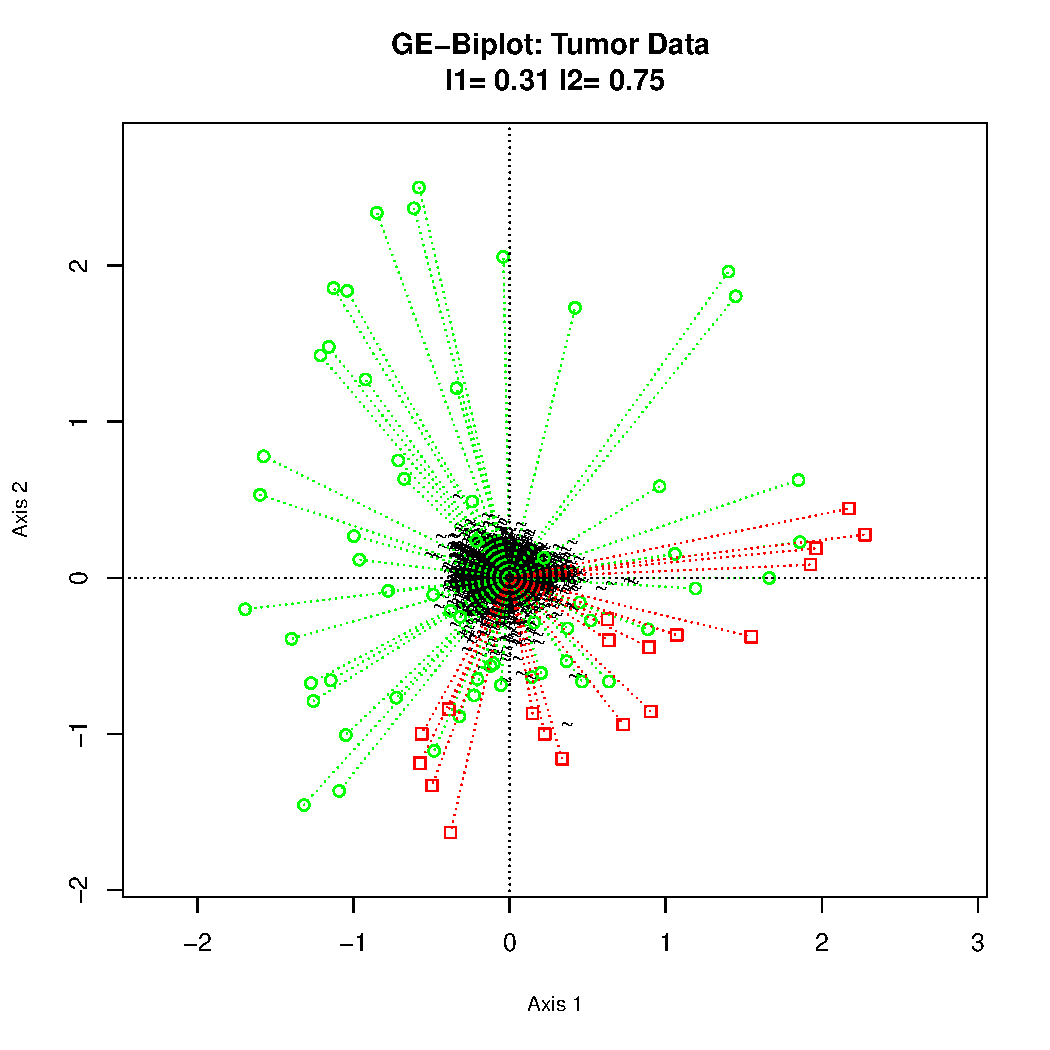
\includegraphics[width=1.5in, height=1.5in]{images/final_graphs/LYMPHOMA_BIPLOT}\newline
						\ConstrainedBox{0.25in}{1.75in}
						{
							Standard Biplot
						}
					\end{center}
				}
			\end{column}
		\end{columns}
		
	\end{frame}
	
	\begin{frame}[t]
		\frametitle{Biplot Interpretations}
		\framesubtitle{Err... now what?}
	
		\only<1>
		{
		\large
		\begin{block}{\vspace{-0.5in}}
			Reading a biplot is \emph{intuitive} \underline{after} you grasp the concepts. 	
		\end{block}
		\raggedright Until then...
		\begin{center}
			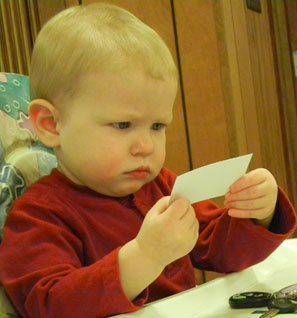
\includegraphics[height=1.5in]{images/confused}	
		\end{center}
		\raggedleft ...It's rather confusing.
		}
		
		\only<2>
		{
			\begin{columns}
				\begin{column}{1.5in}
					Some image
				\end{column}
				\begin{column}{2.5in}
					\begin{block}{Upregulation}	
						Genes that lie \textbf{close} to a cluster of samples are more highly expressed (upregulated) in that cluster of samples versus others.
					\end{block}
				\end{column}
			\end{columns}
			\vspace{0.30in}
			\begin{columns}
				\begin{column}{1.5in}
					Some image
				\end{column}
				\begin{column}{2.5in}
					\begin{block}{Downregulation}
						Likewise, Genes that lie \textbf{far away} from a cluster of samples are less expressed (downregulated) in that cluster of samples versus others.
					\end{block}
				\end{column}
			\end{columns}
		}
		
		\only<3>
		{
			\vspace{0.75in}
			\begin{columns}
				\begin{column}{1.5in}
					Some image
				\end{column}
				\begin{column}{2.5in}
					\begin{block}{Differential Expression}
						Genes that are \textbf{further away} from the origin are more differentially expressed than genes that are \textbf{closer} to the origin.
					\end{block}
				\end{column}
			\end{columns}
		}
		
		\only<4>
		{
			% CITE: http://www.ggebiplot.com/hs40.htm
			\begin{center}
				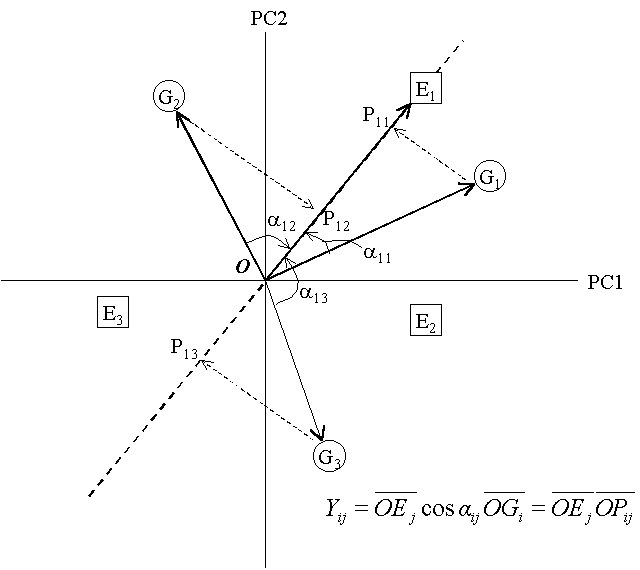
\includegraphics[width=2.0in]{images/inner_product_property_biplot}
			\end{center}
			
			\begin{block}{Inner Product Property}
				some kind of explanation lol
			\end{block}
		}
		
		\only<5>
		{
			% CITE: http://www.ggebiplot.com/hs40.htm
			\begin{center}
				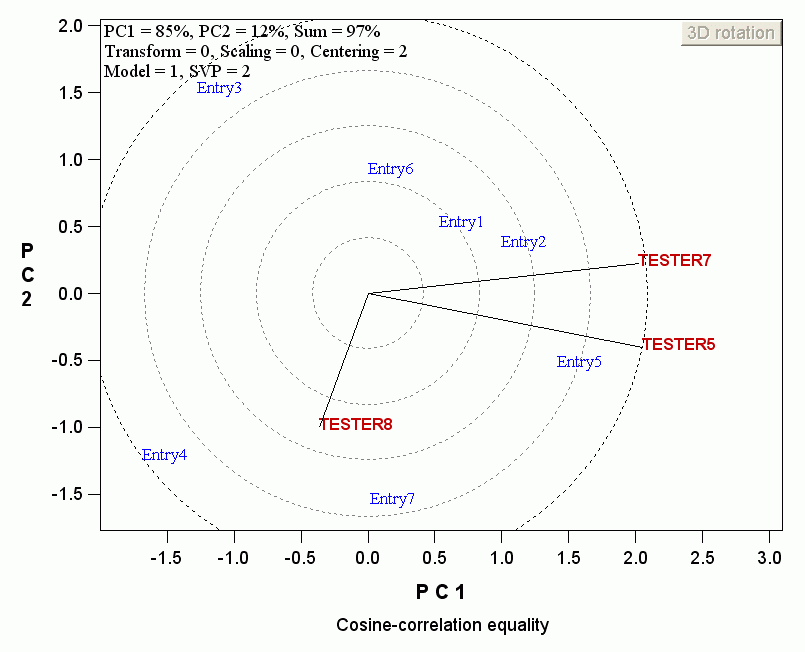
\includegraphics[width=2.0in]{images/cosine_correlation_property_biplot}	
			\end{center}
			
			\begin{block}{Cosine Correlation Property}
						some kind of explanation lol
			\end{block}
			
		}
		
	\end{frame}
	
	
	\section{Analysis}
	
	\begin{frame}[t]
		\frametitle{Analysis of Genes}
		\framesubtitle{Exploring and Validating Highly Differential Genes}
		\begin{block}{\vspace{-0.5in}}
			\alert{Still currently a work in progress.}
		\end{block}
		We hope to verify and expand on Reverter et al.'s findings.
		
		\only<2>
		{
			\begin{block}{Notable Tumor Genes}
				
			\end{block}
		}
		
		\only<3>
		{
			\begin{block}{Notable Leukemia Genes}
				
			\end{block}
		}
		
		\only<4>
		{
			\begin{block}{Notable Lymphoma Genes}
				
			\end{block}
		}
	\end{frame}	
	
	\section{Program}
	
	\begin{frame}
	
	\begin{columns}
		\begin{column}{2.4in}
			
			\vspace{0.25in}
			\begin{center}
				\raggedleft
				\only<1-3>
				{
					
\includegraphics[width=2.25in]{images/python_logo}
				}
				\only<4-9>
				{
					
\includegraphics[width=2.25in]{images/python_logo_dimmed}
				}
			\end{center}
			\begin{center}
				\emph{\Huge \&}
			\end{center}
			\begin{center}
				\raggedright
				\only<1-3>
				{
					
\includegraphics[width=1.300in]{images/R_logo_dimmed}	
				}
				\only<4-9>
				{
					
\includegraphics[width=1.300in]{images/R_logo}	
				}
			\end{center}
			\begin{center}
				\emph{Went together like cookies and milk}
			\end{center}
			
		\end{column}
		\begin{column}{1.6in}	
			\begin{exampleblock}{Implementation}
				\begin{itemize}
					\item
					{
						\color<4-9>{blockgray}
						{
							\textbf{Python}
						}
						\begin{itemize}
							\item[$\rightarrow$]
							{
							
								\color<1,3-9>{blockgray}{Initial Prototyping}
							}
							\item[$\rightarrow$]
							{
								\color<1-2,4-9>{blockgray}{Manipulation of raw data
								into kosher formats for R}
							}
						\end{itemize}
					}
					\item
					{
						\color<1-3>{blockgray}
						{
							\textbf{R}
						}
					\begin{itemize}
						\item[$\rightarrow$]
						{
							\color<1-4,6-9>{blockgray}{KPCA Implementation}
						}
						\item[$\rightarrow$]
						{
							\color<1-5,7-9>{blockgray}{JUMP Algorithm}
						}
						\item[$\rightarrow$]
						{
							\color<1-6,8-9>{blockgray}{Crossvalidation}
						}
						\item[$\rightarrow$]
						{
							\color<1-7,9>{blockgray}{Biplots}
						}
						\item[$\rightarrow$]
						{
							\color<1-8>{blockgray}{Analysis}
						}
					\end{itemize}
					}
				\end{itemize}
			\end{exampleblock}
		\end{column}
	\end{columns}
	
	\end{frame}
	
	
	\section{Insights}
	
	\begin{frame}[t]
		\frametitle{Insights / Reflections}
		\only<1-3>
		{
			{\huge \sc The Good}
			\begin{itemize}
				\item
				{
					\color<2-3>{gray10percent}
					{
						\footnotesize
						Datasets were readily available
					}
					\vspace{-0.2in}
					\begin{columns}
						\begin{column}{0.5in}
							%NOTE: FOR SPACING ONLY
						\end{column}
						% Visually looks like indented block without title
						\begin{column}{3.5in}
							
							\begin{block}{\vspace{-0.5in}}
							\begin{columns}
								\begin{column}{1.0in}
									\begin{center}
										\only<1>
										{
											
\includegraphics[width=1in]{images/assemblyrequired}
										}
										\only<2-3>
										{
											
\includegraphics[width=1in]{images/assemblyrequired_dimmed}
										}
									\end{center}
								\end{column}
								\begin{column}{2.5in}
									\color<2-3>{blockgray}
									{
									\footnotesize
									Some formatting and massaging was needed
									}
								\end{column}	
							\end{columns}
							\end{block}
						\end{column}
					\end{columns}
					
				}
				\item 
				{
					\color<1,3>{gray10percent}
					{
						\footnotesize
						Good applied use of R which is extremely useful for data mining.
					}
					\vspace{-0.3in}
					\begin{columns}
						\begin{column}{0.5in}
							%NOTE: FOR SPACING ONLY
						\end{column}
						% Visually looks like indented block without title
						\begin{column}{3.5in}
							
							\begin{block}{\vspace{-0.5in}}
							\begin{columns}
								\begin{column}{1.0in}
									\begin{center}
									\only<2>
									{
										
\includegraphics[width=1in]{images/bioconductor}	
									}
									\only<1,3>
									{
										
\includegraphics[width=1in]{images/bioconductor_dimmed}
									}
									\end{center}
									
								\end{column}
								\begin{column}{2.5in}
									\color<1,3>{blockgray}
									{
									\footnotesize
									{\sc Bioconductor} package provides excellent bioinformatics packages for R.
									Well worth a look!
									\newline
									\newline
									We used code of theirs for our {\sc Biplots}.
									}
								\end{column}	
							\end{columns}
							\end{block}
						\end{column}
					\end{columns}
				
				}
				\item 
				{
					\color<1-2>{gray10percent}
					{
						\footnotesize
						Awesome introduction to exploratory statistics.
					}
					\vspace{-0.2in}
					\begin{columns}
						\begin{column}{0.5in}
							%NOTE: FOR SPACING ONLY
						\end{column}
						% Visually looks like indented block without title
						\begin{column}{3.5in}
							
							\begin{block}{\vspace{-0.5in}}
							\begin{columns}
								\begin{column}{1.0in}
									\begin{center}
										\only<1-2>
										{
											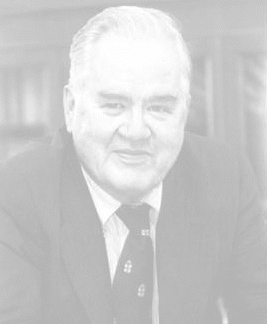
\includegraphics[width=0.60in]{images/johntukey_dimmed}	
										}
										\only<3>
										{
											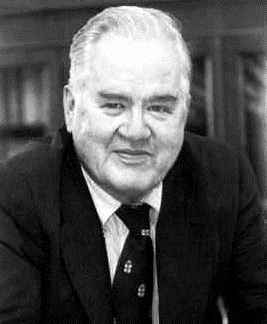
\includegraphics[width=0.60in]{images/johntukey}
										}
									\end{center}
								\end{column}
								\begin{column}{2.5in}
									\color<1-2>{blockgray}
									{
									\footnotesize
									As the famous statistician, John Tukey once said:
									\newline
									``Visually examine your data set \emph{then}
									formulate the hypothesis you wish to test"	
									}
								\end{column}	
							\end{columns}
							\end{block}
						\end{column}
					\end{columns}
				}
			\end{itemize}
		}
		\only<4-5>
		{
			{\huge \sc The Bad}
			\begin{itemize}
				\item 
				{
					\color<5>{gray10percent}
					{
						\footnotesize
						Literature on biplots was very esoteric.
					}
					\vspace{-0.2in}
					\begin{columns}
						\begin{column}{0.5in}
							%NOTE: FOR SPACING ONLY
						\end{column}
						% Visually looks like indented block without title
						\begin{column}{3.5in}
							
							\begin{block}{\vspace{-0.5in}}
							\begin{columns}
								\begin{column}{1.0in}
									\begin{center}
										\only<5>
										{
											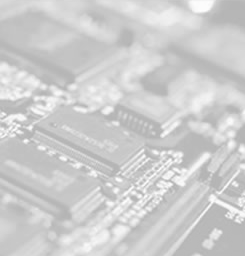
\includegraphics[width=0.75in]{images/computer_chip_dimmed}	
										}
										\only<4>
										{
											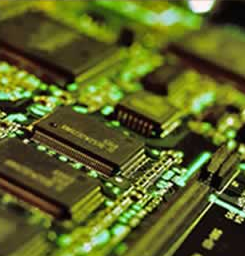
\includegraphics[width=0.75in]{images/computer_chip}
										}
									\end{center}
								\end{column}
								\begin{column}{2.5in}
									\color<5>{blockgray}
									{
									\footnotesize
									Definitely \underline{not} written for {\sc engineers}, {\sc applied mathematicians}, etc.
									\newline\newline
									Explanations are usually in terms of domain specific terminology such as {\sc Breeders}, {\sc Geneticists}, and {\sc Agronomists}.
									}
								\end{column}	
							\end{columns}
							\end{block}
						\end{column}
					\end{columns}
				}
				\item 
				{
					\color<4>{gray10percent}
					{
						\footnotesize
						The datasets were very computationally expensive as we expected.
					}
					\vspace{-0.3in}
					\begin{columns}
						\begin{column}{0.5in}
							%NOTE: FOR SPACING ONLY
						\end{column}
						% Visually looks like indented block without title
						\begin{column}{3.5in}
							
							\begin{block}{\vspace{-0.5in}}
							\begin{columns}
								\begin{column}{1.0in}
									\begin{center}
										\only<4>
										{
											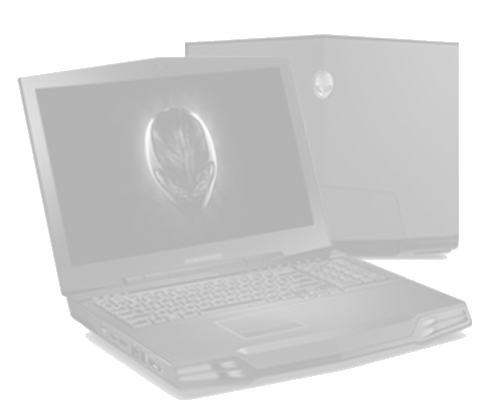
\includegraphics[width=0.75in]{images/alienware_dimmed}	
										}
										\only<5>
										{
											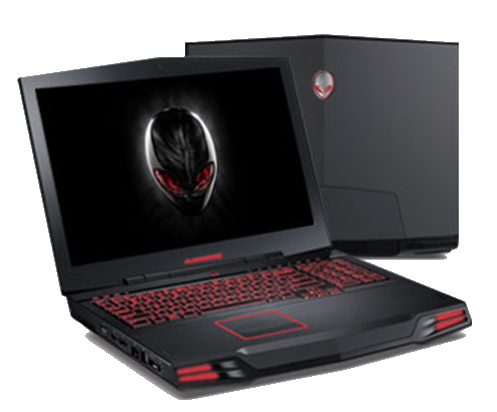
\includegraphics[width=0.75in]{images/alienware}
										}
									\end{center}
								\end{column}
								\begin{column}{2.5in}
									\color<4>{blockgray}
									{
										\footnotesize
										Some datasets locked up all computers but
										an {\sc Alienware M17x} that one of us had.
									}
								\end{column}	
							\end{columns}
							\end{block}
						\end{column}
					\end{columns}
				}
			\end{itemize}
		}
		\only<6-8>
		{
			{\huge \sc The Ugly}
			\begin{itemize}		
				\item 
				{
					\color<7-8>{gray10percent}
					{
						\footnotesize
						Cross validation methodology was too vague to be replicated.
					}
					\vspace{-0.2in}
					\begin{columns}
						\begin{column}{0.5in}
							%NOTE: FOR SPACING ONLY
						\end{column}
						% Visually looks like indented block without title
						\begin{column}{3.5in}
							
							\begin{block}{\vspace{-0.5in}}
							\begin{columns}
								\begin{column}{1.0in}
									\begin{center}
										\only<7-8>
										{
											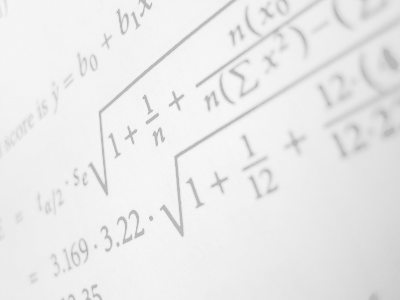
\includegraphics[width=0.75in]{images/cross_validate_dimmed}	
										}
										\only<6>
										{
											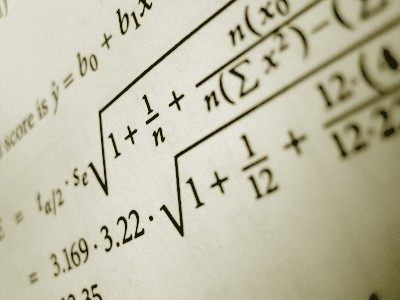
\includegraphics[width=0.75in]{images/cross_validate}
										}
									\end{center}
								\end{column}
								\begin{column}{2.5in}
									\color<7-8>{blockgray}
									{
										\footnotesize
										Required research of applicable cross-validation techniques.
									}
								\end{column}	
							\end{columns}
							\end{block}
						\end{column}
					\end{columns}
				}
				\item 
				{
					\color<6,8>{gray10percent}
					{
						\footnotesize
						No KPCA-Biplot code freely available 
					}
					\vspace{-0.2in}
					\begin{columns}
						\begin{column}{0.5in}
							%NOTE: FOR SPACING ONLY
						\end{column}
						% Visually looks like indented block without title
						\begin{column}{3.5in}
							
							\begin{block}{\vspace{-0.5in}}
							\begin{columns}
								\begin{column}{1.0in}
									\begin{center}
										\only<6,8>
										{
											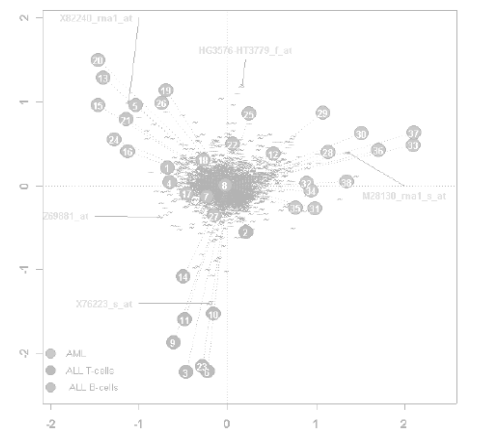
\includegraphics[width=0.75in]{images/kpca_biplot_dimmed}	
										}
										\only<7>
										{
											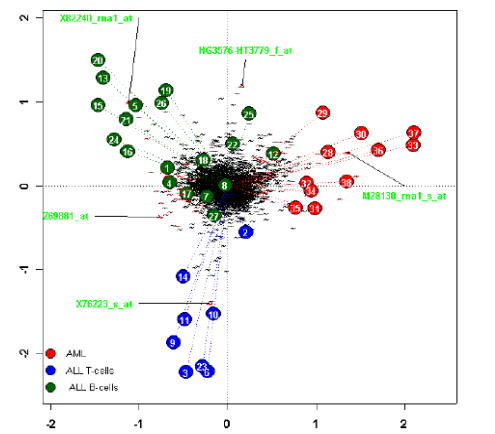
\includegraphics[width=0.75in]{images/kpca_biplot}
										}
									\end{center}
								\end{column}
								\begin{column}{2.5in}
									\color<6,8>{blockgray}
									{
										\footnotesize
										Implemented per instructions of the paper and validated results to ensure correctness.
									}
								\end{column}	
							\end{columns}
							\end{block}
						\end{column}
					\end{columns}
				}
				\item 
				{
					\color<6-7>{gray10percent}
					{
						\footnotesize
						Actual datasets no where in sight just mention of papers.
					}
					\vspace{-0.2in}
					\begin{columns}
						\begin{column}{0.5in}
							%NOTE: FOR SPACING ONLY
						\end{column}
						% Visually looks like indented block without title
						\begin{column}{3.5in}
							
							\begin{block}{\vspace{-0.5in}}
							\begin{columns}
								\begin{column}{1.0in}
									\begin{center}
										\only<6-7>
										{
											
\includegraphics[width=0.60in]{images/search_dimmed}	
										}
										\only<8>
										{
											
\includegraphics[width=0.60in]{images/search}
										}
									\end{center}
								\end{column}
								\begin{column}{2.5in}
									\color<6-7>{blockgray}
									{
										\footnotesize
										Had to search high and low to get datasets that were applicable for our implementation.
									}
								\end{column}	
							\end{columns}
							\end{block}
						\end{column}
					\end{columns}
				}
			\end{itemize}
		}
	\end{frame}
	
	\section{Extensions}
	
	\begin{frame}[t]
		\frametitle{Possible Extensions}
		Authors had no extensions listed or even so much as to a hint on what possible could be done.
		\newline\newline
		Here's some:
		\begin{itemize}
			\item  Algorithm to select highly differentiable genes automatically
			using the intrinsic relationships of biplots
			\item  Algorithm to find the best alpha for biplot
			% EXPLAIN
			\item  Goodness of Fit metrics for biplots
		\end{itemize}
	\end{frame}
	
	\begin{frame}
		\frametitle{That's all folks}
		\framesubtitle{Questions?}
		
		\begin{center}
			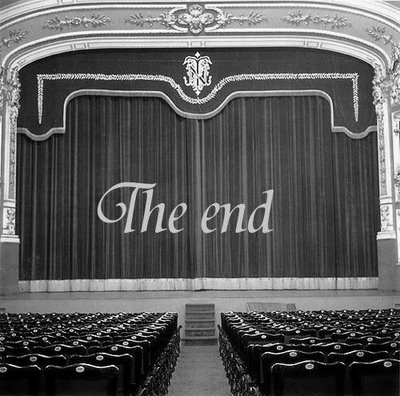
\includegraphics[height=2.75in]{images/end}	
		\end{center}
		
	\end{frame}

	\begin{frame}
		Bib
	\end{frame}
	
\end{document}